Similarly to the \wh{} analysis, for the \zh{} STXS analysis three POIs are measured per SR category for each \ptv{} bin. From the fit, the expected signal strength in the one SFOS category for each \ptv{} bin, listed in order of $\ptv < 75$~GeV, $75 \leq \ptv < 150$~GeV, and $\ptv \geq 150$~GeV, are found to be $\mu = 1.00^{+0.76}_{-0.76}$, $\mu = 1.00^{+0.73}_{-0.73}$, and $\mu = 1.00^{+0.89}_{-0.89}$, and in the two SFOS category are found to be $\mu = 1.00^{+2.15}_{-2.15}$, $\mu = 1.00^{+1.34}_{-1.34}$, and $\mu = 1.00^{+1.38}_{-1.38}$. In the combined \zh{} channel, the expected $\mu$ values are found to be $\mu = 1.00^{+0.73}_{-0.73}$, $\mu = 1.00^{+0.64}_{-0.64}$, and $\mu = 1.00^{+0.74}_{-0.74}$. At the time of writing this thesis, the observed values are still blinded, hence only expected values will be reported.

The impact of statistical and systematic uncertainties on the STXS \zh{} measurement is assessed through the pulls (Appendix~\ref{app:zh_stxs_pull_plots}), the correlations between uncertainties (Appendix~\ref{app:zh_stxs_correlation_plots}), and the systematic ranking plots (Appendix~\ref{app:zh_stxs_ranking_plots}). The NFs for the $ZZ$ CR is found to be $\mathrm{NF}_{ZZ} = 0.94^{+0.03}_{-0.03}$.

% Likelihood scans can be seen in Figure~\ref{fig:zh_stxs_likelihood_scans}.

% \begin{figure}[htp]
%   \centering
%   \subfloat[$0 < \ptv < 75$~GeV.]{
%     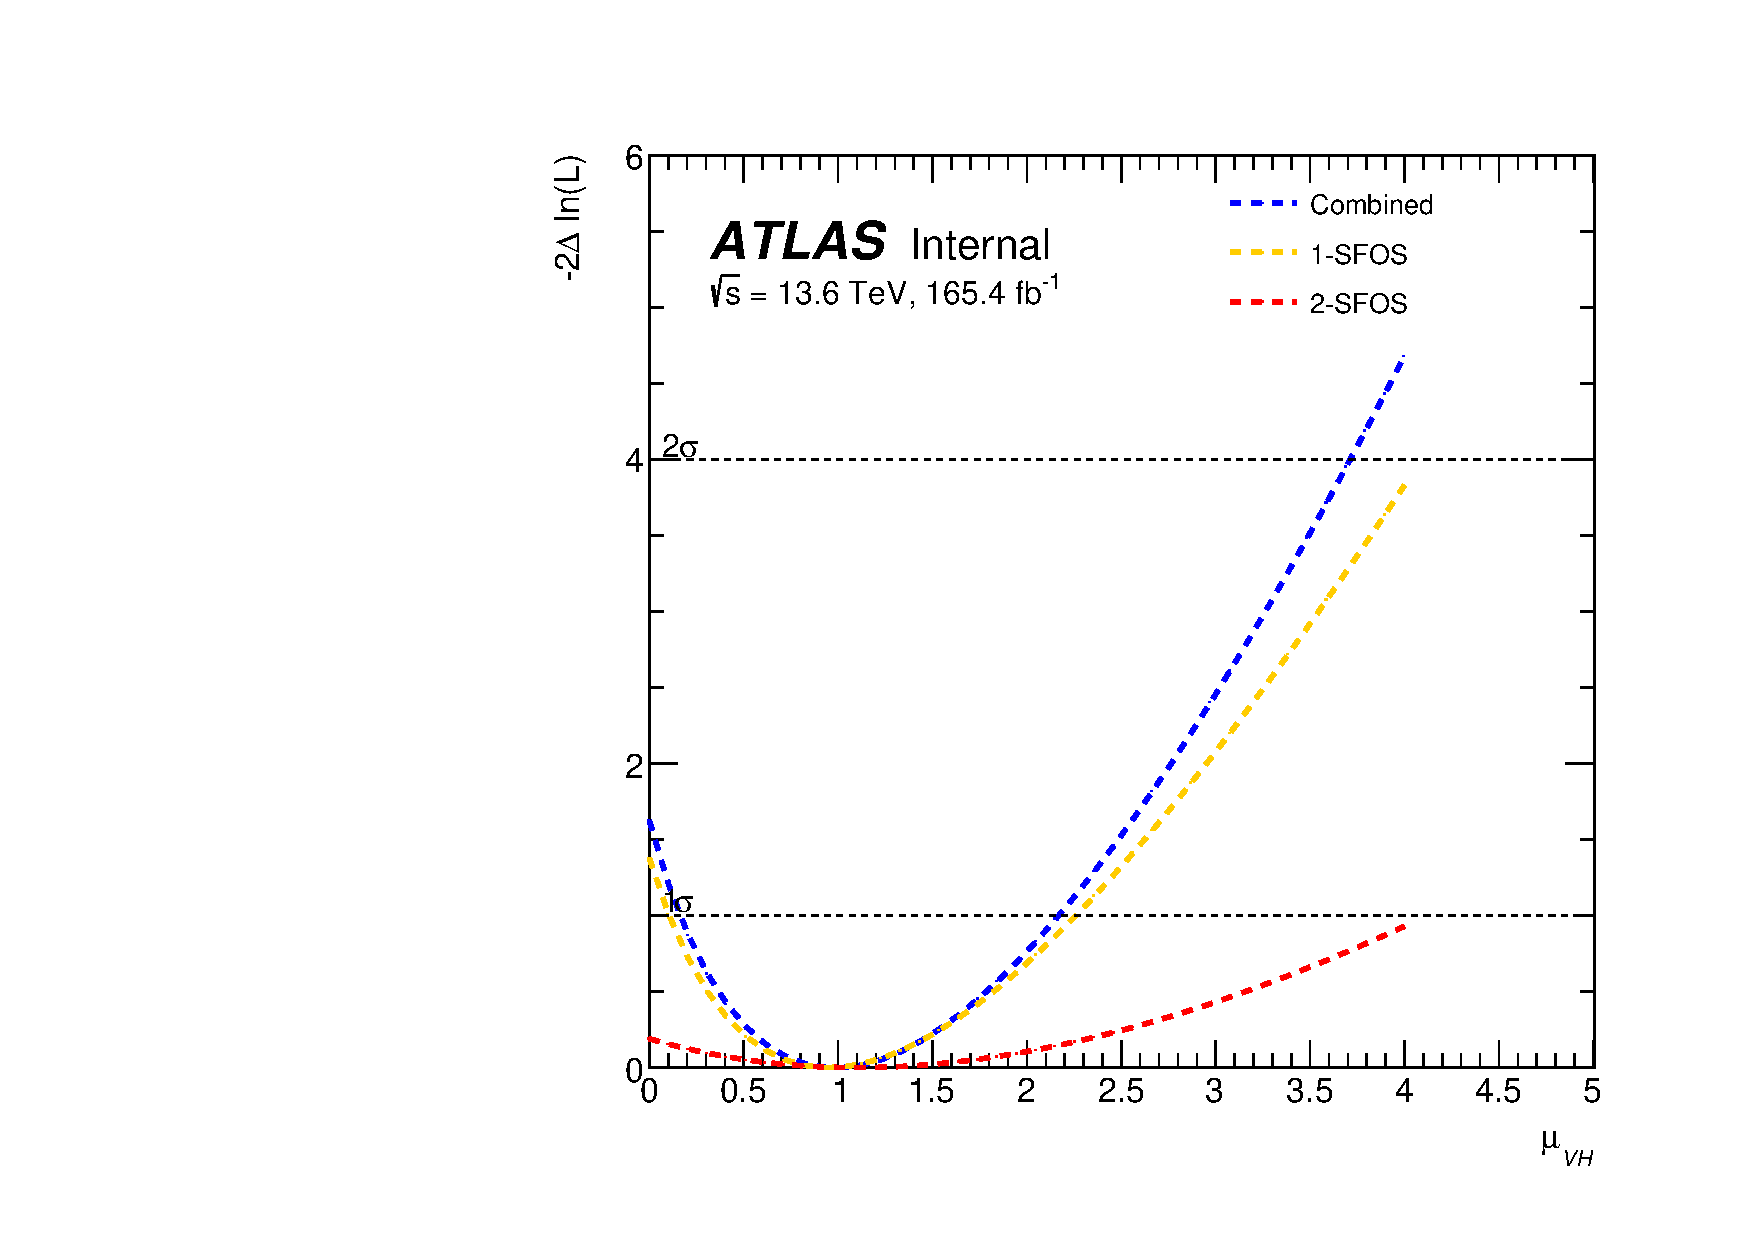
\includegraphics[width=0.45\linewidth]{figures/statistical/scan_plots_0_75_zh.pdf}
%   }
%   \subfloat[$75 \leq \ptv < 150$~GeV.]{
%     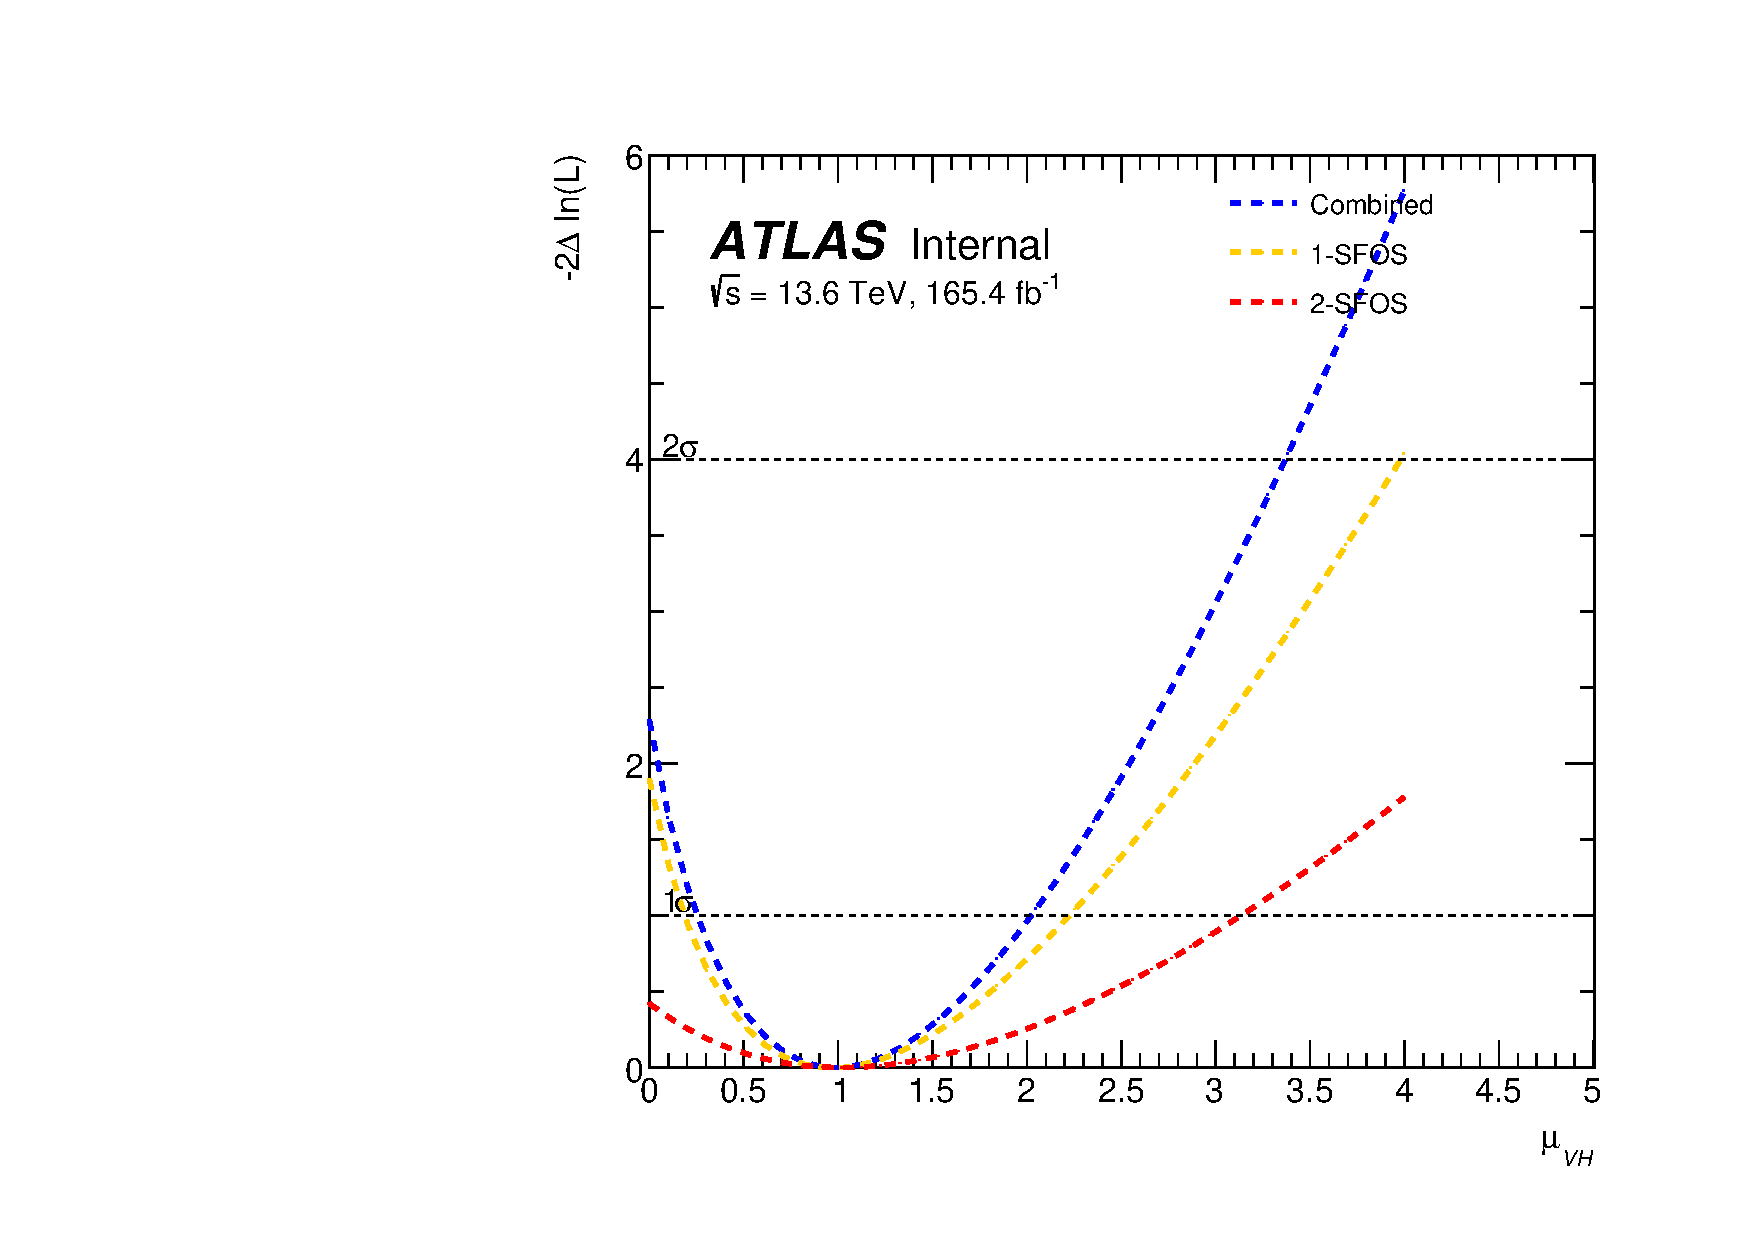
\includegraphics[width=0.45\linewidth]{figures/statistical/scan_plots_75_150_zh.pdf}
%   }\hfill
%   \subfloat[$\ptv \geq 150$~GeV.]{
%     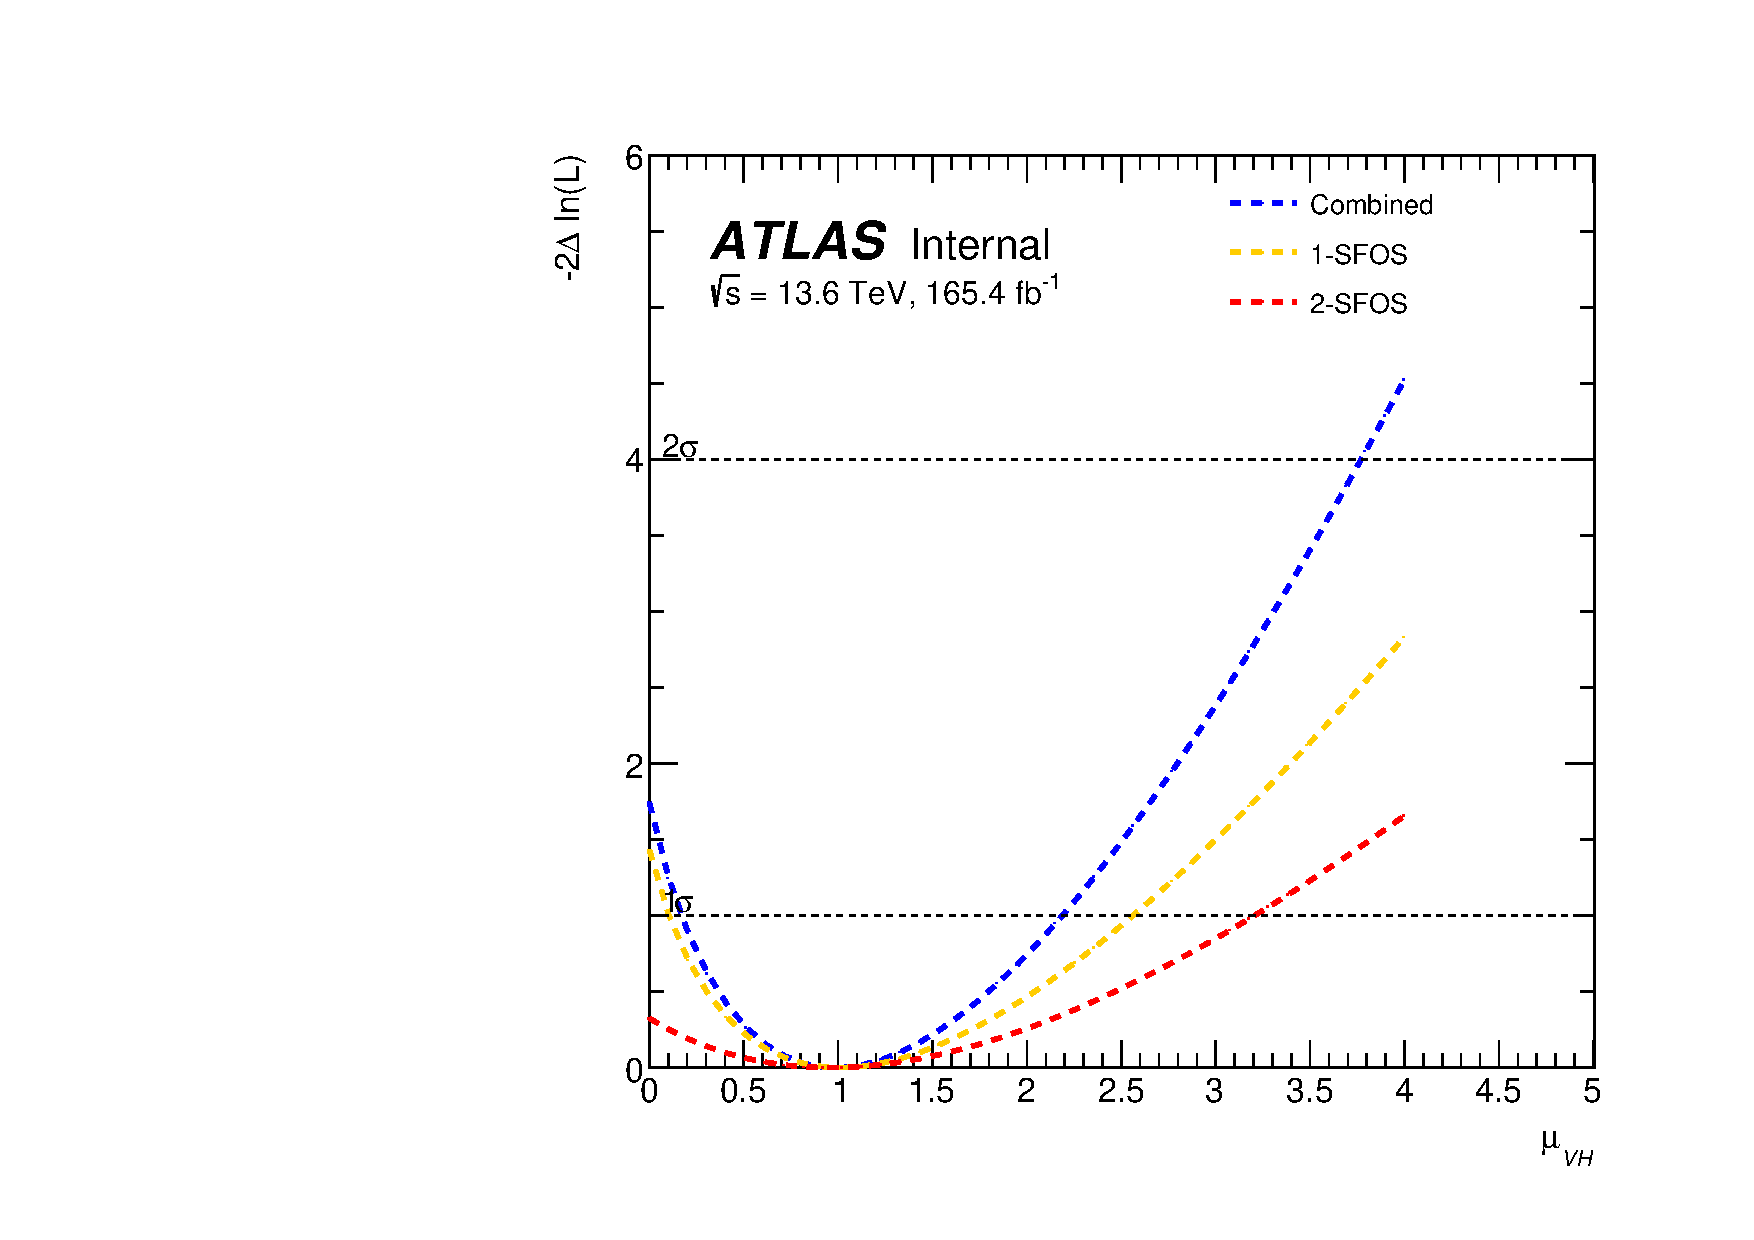
\includegraphics[width=0.45\linewidth]{figures/statistical/scan_plots_150_inf_zh.pdf}
%   }
%   \caption{Expected likelihood scans for \zh{} SR split by STXS bin.}\label{fig:zh_stxs_likelihood_scans}
% \end{figure}

All results from the \zh{} STXS channels are summarized in Tables~\ref{tab:zh_stxs_results_summary}.

\begin{table}[htp]
    \centering
    \begin{tabular}{l|c|c|c}
      \hline
      \multicolumn{4}{c}{\textbf{Results Summary}} \\
      \hline
      \multicolumn{1}{c|}{\textbf{Category}} & \multicolumn{3}{c}{\textbf{STXS Bins}} \\
      & $\ptv < 75$~GeV & $75 \leq \ptv < 150$~GeV & $\ptv \geq 150$~GeV \\
      \hline
      $\mu_{WH}$ (Expected, one SFOS) & $1.00^{+0.76}_{-0.76}$ & $1.00^{+0.73}_{-0.73}$ & $1.00^{+0.89}_{-0.89}$ \\
      \hline
      $\mu_{WH}$ (Expected, two SFOS) & $1.00^{+2.15}_{-2.15}$ & $1.00^{+1.34}_{-1.34}$ & $1.00^{+1.38}_{-1.38}$ \\
      \hline
      $\mu_{WH}$ (Expected, Combined) & $1.00^{+0.73}_{-0.73}$ & $1.00^{+0.64}_{-0.64}$ & $1.00^{+0.74}_{-0.74}$ \\
      \hline
    \end{tabular}
    \caption{Summary of the expected signal strengths for the \zh{} STXS fit, broken down by \ptv{} bin and channel.}\label{tab:zh_stxs_results_summary}
  \end{table}